\section{Methodik}\label{chap:Methodik}

Es werden zunächst die verwendeten Netztopologien sowie deren Clusterung zur Bestimmung repräsentativer Netze, anhand welcher die Untersuchungen vorgenommen werden, beschrieben und vorgestellt.
Anschließend werden mit Hilfe des Software Tools \gls{SIMBEV} Fahrtprofile von \glspl{EPKW} erstellt und die untersuchten Ladestrategien beschrieben.
Damit der Ladebedarf in die Netzmodelle integriert werden kann, muss dieser anschließend räumlich auf eine entsprechende georeferenzierte Ladeinfrastruktur verteilt werden.
Abschließend erfolgt eine Beschreibung der Methodik zur Bestimmung von Netzproblemen und der Ermittlung des Abregelungsbedarfs im Netzgebiet mit Hilfe des Open Source Tools \gls{EDISGO}.


\subsection{Verwendete Verteilnetztopologien}\label{chap:dingo_theo}

Eine der Grundlagen für die Nutzung des Netzplanungsinstruments \glspl{EDISGO} sind die zu untersuchenden Netztopologien der \gls{MS}- und \gls{NS}-Ebene.
Aufgrund der mangelnden Datenlagen von realen Netztopologien, wird auf synthetisch erzeugte Netztopologien zurückgegriffen, die innerhalb des \gls{OPENEGO} Projektes \cite{Mueller2019} mit Hilfe des Open Source Tools \gls{DINGO} erzeugt wurden.
Das Tool ist in der Lage ländliche und suburbane Netzstrukturen für Gesamtdeutschland zu synthetisieren und kann auf GitHub \cite{dingo2019} öffentlich eingesehen und frei verwendet werden.
Weiterhin findet sich auf Read the Docs \cite{dingo-docs2019} eine ausführliche Dokumentation.\medskip

Die Synthetisierung der Netztopologien ist nicht Teil dieser Masterarbeit und erfolgte innerhalb des \gls{OPENEGO} Projektes \cite{Mueller2019}.
Die Netztopologien werden auf der Datengrundlage des Jahres \num{2015} gebildet und entsprechend ausgebaut.
Urbane Netzgebiete können derzeit nicht durch \gls{DINGO} abgebildet werden und werden deshalb innerhalb dieser Masterarbeit nicht betrachtet. \medskip

In der konventionellen Netzplanung werden Betriebsmittel in der Regel überdimensioniert ausgelegt, um eine möglichst lange Betriebszeit zu garantieren.
Da die Netzgebiete des \gls{OPENEGO} Projektes so ausgebaut werden, dass die Versorgungsaufgabe des Jahres \num{2015} möglichst genau übernommen werden kann, werden die Netzgebiete zusätzlich ausgebaut.
Es wird angenommen, dass die Betriebsmittel mit einem Überdimensionierungsfaktor für die Scheinleistungs- bzw. Stromstärkenbelastbarkeit von mindestens \num{1.4} geplant werden und werden entsprechend ausgebaut.
Dies gilt sowohl für die Transformatorstationen als auch die Kabel innerhalb des Netzgebietes.
Die verwendeten Betriebsmittel können der Dokumentation \glspl{EDISGO} \cite{edisgoDocs2017a} entnommen werden.
Sollte die maximal auftretende Scheinleistungsbelastung einer Transformator-Station größer sein als der größte verfügbare Transformator, so werden so viele Transformatoren wie nötig parallel betrieben, um den Anforderungen gerecht zu werden.


\paragraph{Mittelspannung:}

Die einzelnen \gls{MS}-Netze werden alle als offene Ringnetze betrieben.
Im städtischen Bereich werden hauptsächlich Erdkabel mit einer Nennspannung von \SI{10}{\kv} eingesetzt, während im ländlichen Raum größtenteils Freileitungen mit einer Nennspannung von \SI{20}{\kv} eingesetzt werden. \cite{Mueller2019}\medskip

Die Modellierung der Mittelspannungstopologie erfolgt als Tourenplanungsproblem (\gls{CVRP}) in Kombination mit der Beachtung der historisch lastorientierten Entwicklung und den Planungsprinzipien von Verteilnetzen.
Ein besonderer Fokus liegt dabei auf der Beachtung von Leitungsüberlastungen und Verletzungen des Spannungsbandes.
Eine genau Beschreibung der Methodik findet sich in \textit{The eGo grid model} \cite{Amme2018}.


\paragraph{Niederspannung:}

Die \gls{NS}-Ebene wird mit Hilfe von \num{46} Referenznetzsträngen synthetisiert und die einzelnen \gls{NS}-Netze werden als Strahlennetz abgebildet.
Die Referenznetzsträngen stehen jeweils repräsentativ für eine bestimmte Anzahl an Hausanschlüssen innerhalb einer Netzklasse.
Bei den Netzklassen wird zwischen Land-, Dorf- und Vorstadtnetzen unterschieden.
Auf Grundlage der Anzahl an Hausanschlüssen je Ortsnetzstation wird ein Niederspannungsnetz einer Netzklasse zugeordnet.
Die verschiedenen Referenznetzstränge der entsprechenden Netzklasse werden anschließend so miteinander kombiniert, dass für die entsprechende Anzahl an Hausanschlüssen ein typisches Netz generiert wird. \cite{Mueller2019}


\paragraph{K-Means-Clustering}

Innerhalb des \gls{OPENEGO} Projektes \cite{Mueller2019} wurden in Deutschland insgesamt {\color{red} \num{3354}} Netzgebiete identifiziert und mit Hilfe des Open Source Tools \gls{DINGO} synthetisiert.
Bei der Synthese der Netztopologien wurde auf eine hohe räumliche und zeitliche Auflösung des Netzdatenmodells geachtet.
Die große Anzahl an Netzgebieten und die hohe Auflösung führen zu inakzeptabel hohen Rechenzeiten.
Um die Komplexität des Modells zu reduzieren, wurden in  mit Hilfe des \kmeans Referenznetzgebiete ausgewählt, die stellvertretend für eine möglichst große Zahl an Netzgebieten stehen.
Das \kmean wurde im Rahmen des \gls{OPENEGO} Projektes \cite{Mueller2019} entwickelt und wurde innerhalb \textit{E-Mobility Study} \cite{Schachler} unverändert angewendet.
Innerhalb dieser Arbeit soll eine Teilmenge der ermittelten \num{15} Netzgebiete mit stark unterschiedlichen Charakteristiken untersucht werden.
An dieser Stelle soll das grundlegende Vorgehen erläutert werden. \medskip

Grundlage des \kmeans bildet der \gls{EMA} des Python Paketes \textit{scikit learn}. \cite{scikit-learn2011}
Hierbei kann jedes \gls{MS}-Netz durch die Definition mehrerer numerischer Attribute als Punkt im mehrdimensionalen Raum beschrieben werden.
Der Algorithmus bildet anschließend eine vorgegebene Anzahl an Clustern $k$ durch die Minimierung der Summe der quadrierten gewichteten euklidischen Abstände zwischen den originalen Netzknoten und den Clusterzentren.
Für die Bildung der Cluster werden die folgenden vier Attribute verwendet, um die einzelnen \gls{MS}-Netze zu repräsentieren:

\begin{itemize}
	\item Entwicklung der installierten \gls{PV}-Kapazitäten
	\item Entwicklung der installierten Wind-Kapazitäten
	\item Spitzenlast durch \glspl{WP}
	\item Spitzenlast durch \gls{EPKW}
\end{itemize}

Die Regionalisierung der \gls{PV}-, Wind- und \gls{WP}-Kapazitäten erfolgt nach \autoref{chap:Szenariorahmen}.
Da die Simulation aller \gls{EPKW} aufgrund der großen Anzahl nicht für jedes \gls{MS}-Netzgebiet durchgeführt werden kann, muss die Spitzenlast durch \gls{EPKW} bereits im Voraus abgeschätzt werden.
So wird angenommen, dass nach den Hochlaufzahlen des Antriebswende-Szenarios jeder \gls{PKW} durch einen \gls{EPKW} ersetzt wird und jeder \gls{EPKW} im Jahr \SI{12000}{\km} zurücklegt.
Anhand eines durchschnittlichen Verbrauches von \SI{20}{\kwhkm} wird anschließend der Ladebedarf je Gemeinde abgeschätzt.
Anschließend wird der Ladebedarf mit einem beispielhaften Lastprofil auf die Netzgebiete anhand des Flächenanteils der Gemeinde im Netzgebiete verteilt.


\paragraph{Auswahl repräsentativer Verteilnetztopologien:}

Auf der \gls{MS}-Ebene gibt es {\color{red} \num{3591}} Netzgebiete mit einer mittleren Fläche von \SI{99}{\km\squared}.
\autoref{fig:grid_176_map} zeigt den Aufbau eines beispielhaften Mittelspannungsnetzes, welches mit Hilfe von \gls{DINGO} erzeugt wurde und innerhalb dieser Arbeit untersucht wird.

\begin{figure}[H]
    \centering
    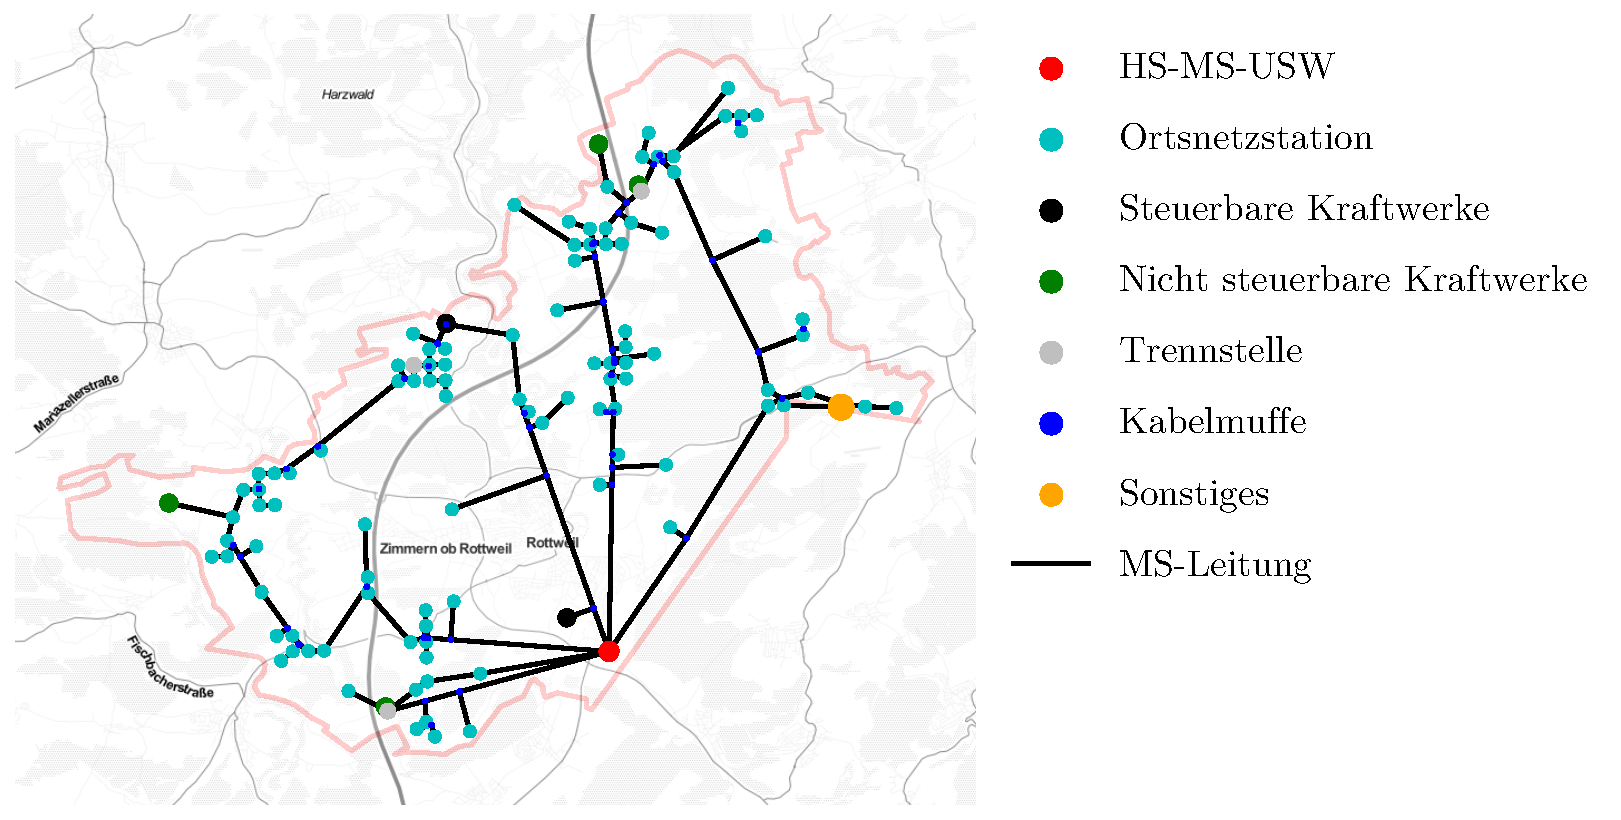
\includegraphics[width=\textwidth]{Bilder/grid_176_map}
    \caption{Beispielhafte Darstellung des MS-Netzes \num{176} mit allen Umspannwerken, Erzeugerkapazitäten und sonstigen Betriebsmitteln}\label{fig:grid_176_map}
\end{figure}

Um mit dieser Arbeit eine Ergänzung zu \textit{E-Mobility Study} \cite{Schachler} zu liefern, werden die Ergebnisse des Clusterings aus \textit{E-Mobility Study} \cite{Schachler} übernommen und von den \num{15} identifizierten repräsentativen Netzgebieten eine Teilmenge untersucht.
So werden jeweils zwei Netzgebiete der Kategorien Wind-, \gls{PV}- und Last-dominiert ausgewählt, die möglichst viele Netzgebiete repräsentieren.
Auf diese Weise wird sichergestellt, dass die Effekte der Netzintegration der Elektromobilität auf möglichst unterschiedliche Netze aufgezeigt werden können.
Insgesamt werden somit sechs Netzgebiete untersucht, die stellvertretend für \num{1842} der {\color{red} \num{3591}} Mittelspannungsnetze stehen.
In \autoref{tab:grid_IDs} finden sich die \glspl{ID} der untersuchten Mittelspannungsnetze und die Anzahl an repräsentierten Netzgebieten.

{
\renewcommand{\arraystretch}{1.2}% grßerer Zeilenabstand
\sisetup{range-phrase=~{--}~}% Gedankenstrich statt "bis" bei SIrange
\begin{table}[H]
	\begin{center}
		\caption{Anzahl der repräsentierten Netzgebiete und Kategorie der untersuchten Mittelspannungsnetze}
		\begin{tabu} to \textwidth {X[1] X[1] X[1, r] }
			\hline
			Netz ID    & Kategorie      & Anzahl repräsentierter Netze \\ \hline
			\num{176}  & PV-dominiert   & \num{413}                    \\
			\num{1056} & PV-dominiert   & \num{197}                    \\
			\num{1690} & Wind-dominiert & \num{141}                    \\
			\num{1811} & Wind-dominiert & \num{78}                     \\
			\num{177}  & Last-dominiert & \num{666}                    \\
			\num{2534} & Last-dominiert & \num{347}                    \\ \hline
		\end{tabu}
		\label{tab:grid_IDs}
	\end{center}
	\vspace{-3mm}%Put here to reduce too much white space after your table
\end{table}
}

In \autoref{fig:bar_representatives} findet sich eine Darstellung der wichtigsten Charakteristika der untersuchten Netzgebiete.
Hierzu zählen die installierten \gls{PV}- und Wind-Kapazitäten, sowie die Spitzenlast der \glspl{EPKW} bei Referenz-Laden im Antriebswende-Szenario und die Spitzenlast des konventionellen Stromverbrauchs inklusive \glspl{WP}.
Weiterhin findet sich in \autoref{fig:map_representatives} eine Karte der repräsentierten Netzgebiete eingeteilt in die Kategorien Wind-, \gls{PV}- und Last-dominiert.

\begin{figure}[H]
    \centering
    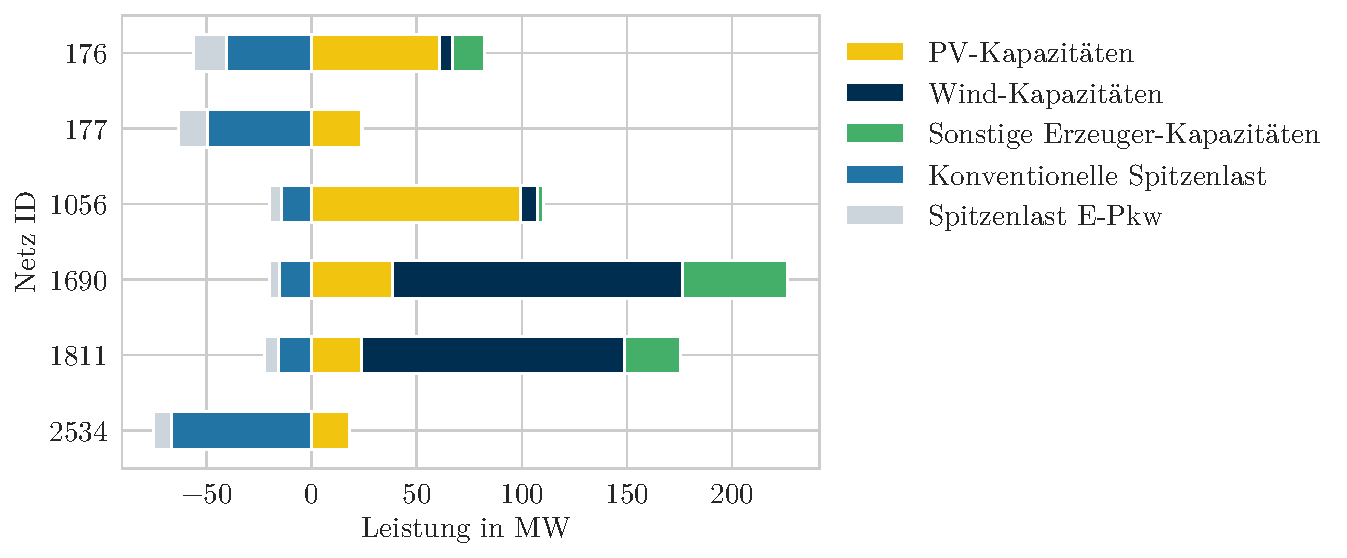
\includegraphics[width=\textwidth]{Bilder/Installed_cap_peak_load_representatives}
    \caption{Kumulierte Wirkleistung von PV-, Wind- und sonstigen Erzeuger-Kapazitäten sowie die kumulierte konventionelle und mobilitätsbedingte Spitzenlast in den Referenznetzgebieten}\label{fig:bar_representatives}
\end{figure}

\begin{figure}[H]
    \centering
    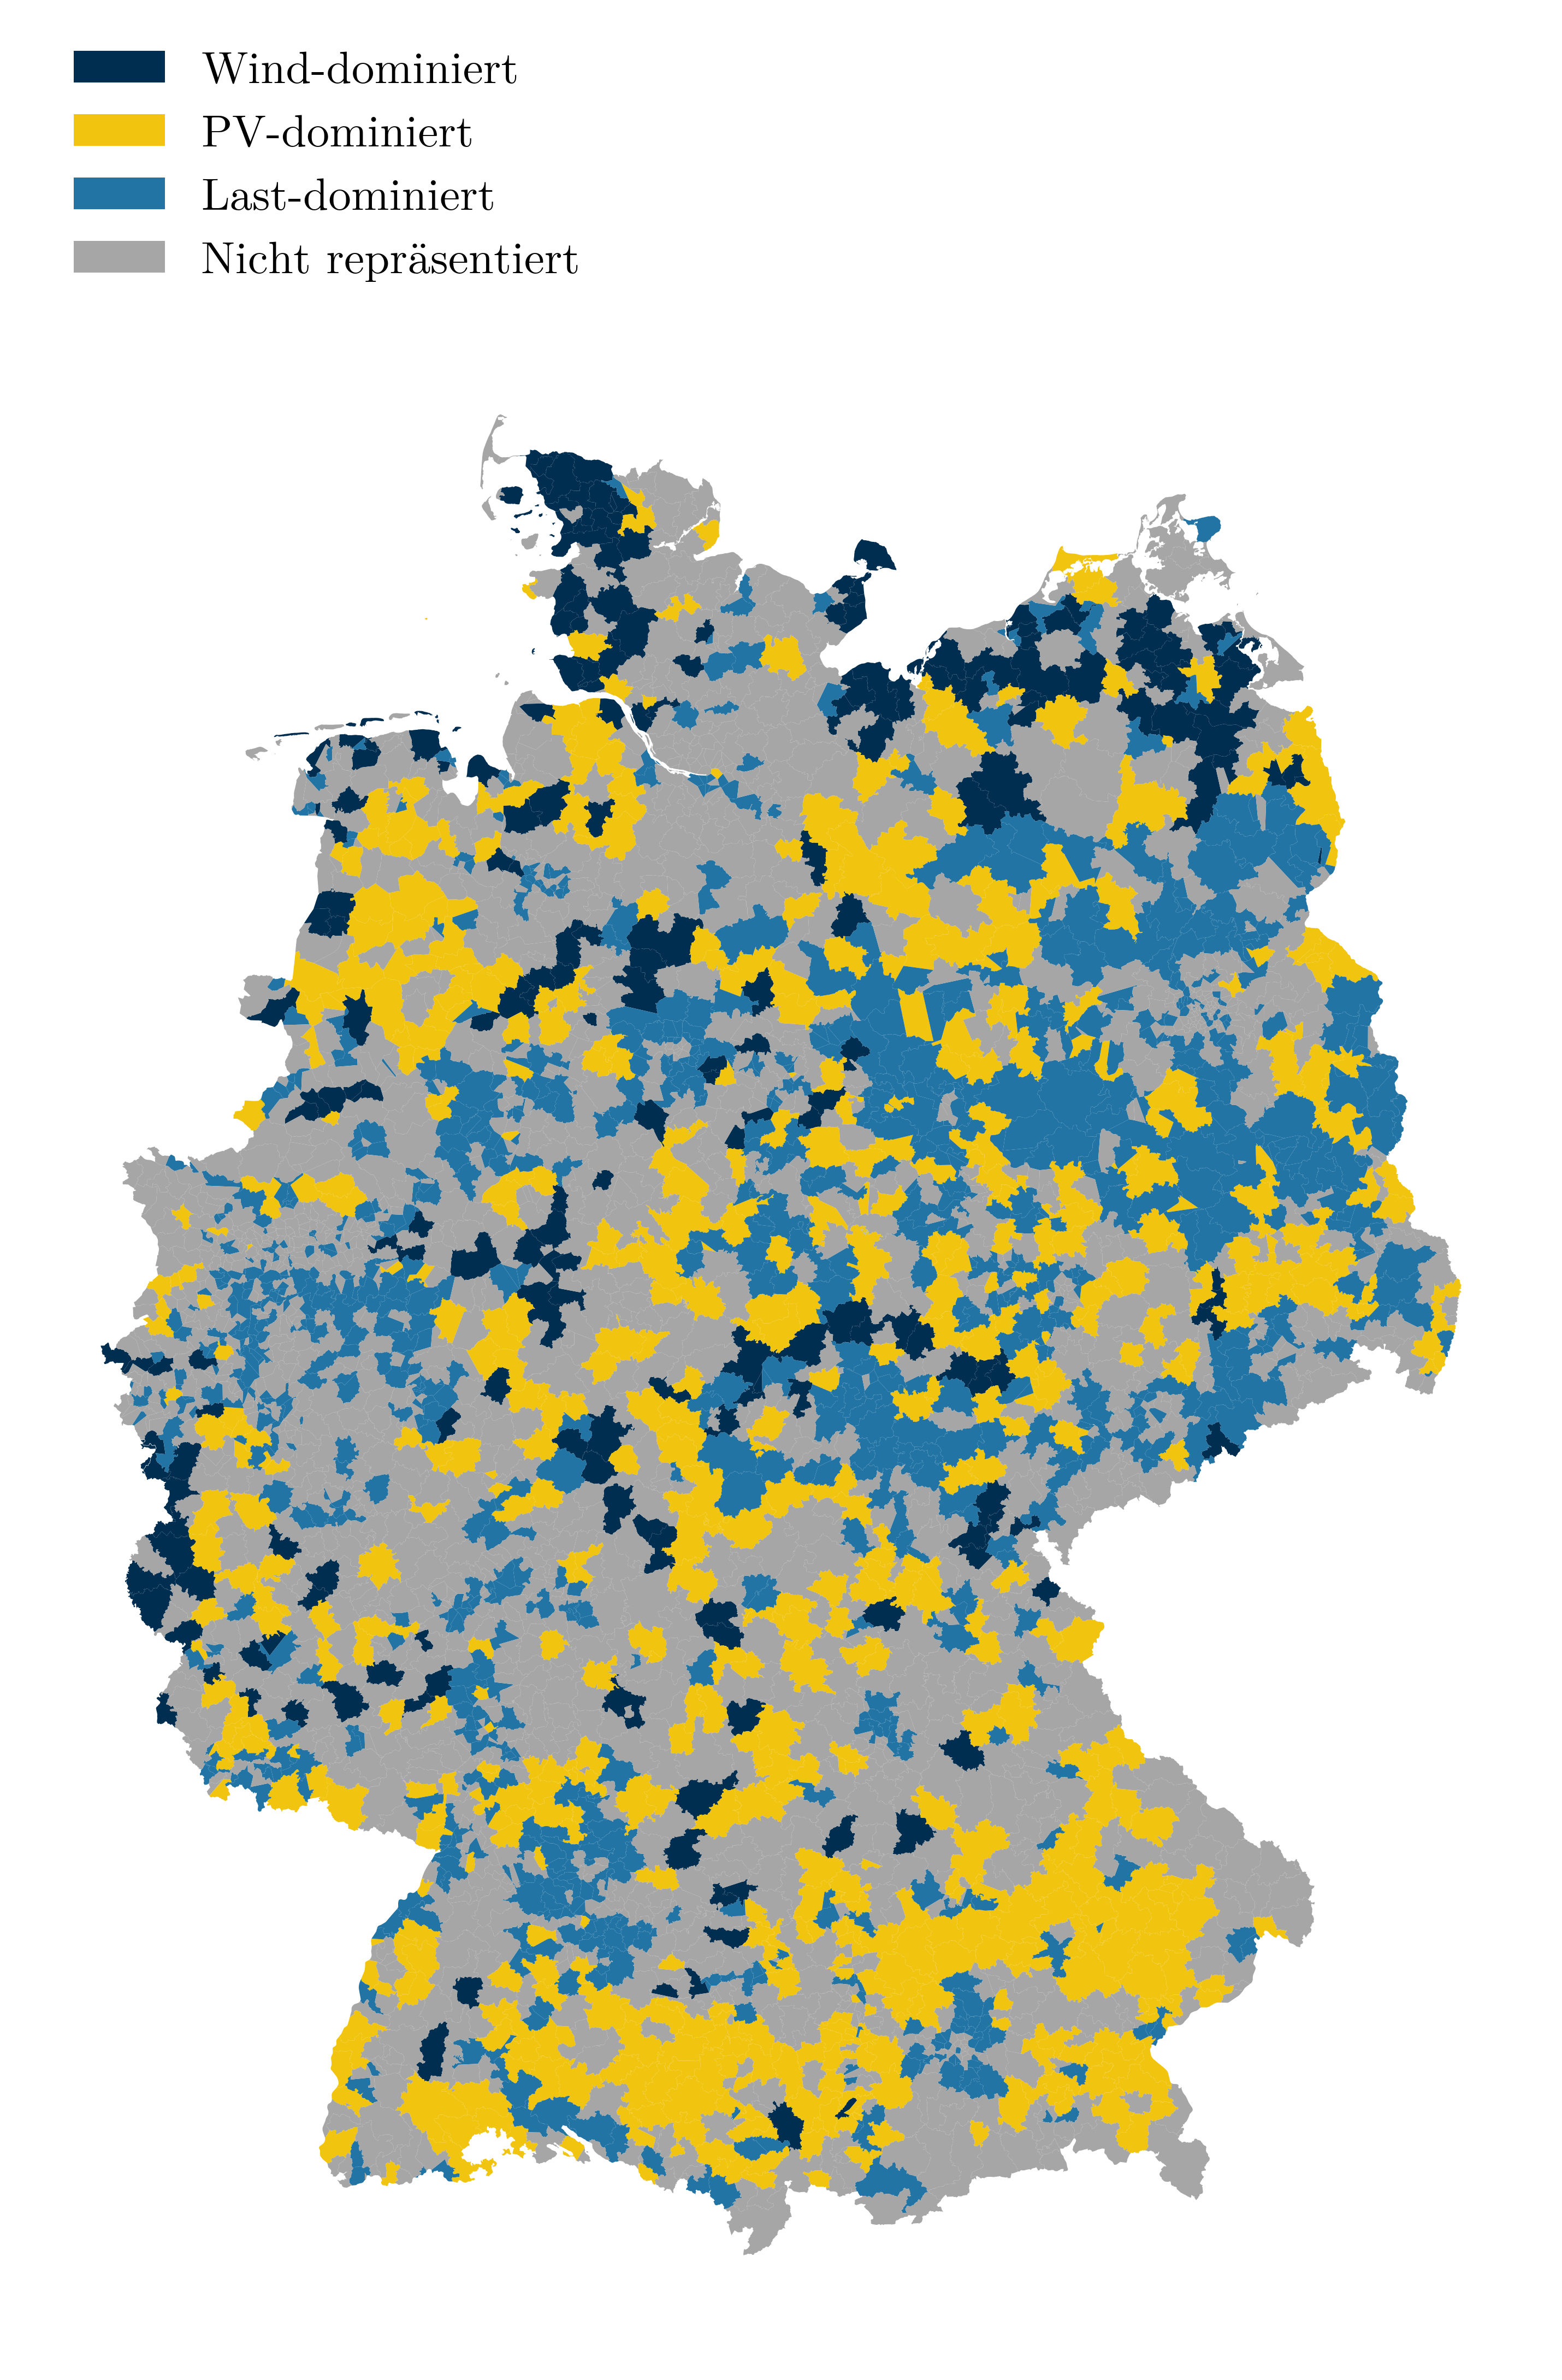
\includegraphics[width=\textwidth]{Bilder/clusters_representatives}
    \caption{Repräsentierte Netzgebiete in Deutschland}\label{fig:map_representatives}
\end{figure}


\subsection{Erstellung der Fahrtprofile von E-Pkw}\label{chap:simbev_theo}

Mit Hilfe des im Rahmen dieser Masterarbeit mitentwickelten Software Tools \gls{SIMBEV} können die Fahrtprofile für eine beliebige Anzahl an Fahrzeugen verschiedener Fahrzeugklassen erstellt werden.
Grundlage \glspl{SIMBEV} bildet die Befragung \gls{MID} \cite{ISGH2017}.
Nachfolgend wird zunächst die Datengrundlage beschrieben und anschließend die Methodik zur Erstellung der Fahrtprofile mit Hilfe \glspl{SIMBEV}.


\subsubsection{Mobilität in Deutschland}\label{chap:MID}

Das Ziel der Befragung \gls{MID} \cite{ISGH2017} ist es, eine Datengrundlage für das alltägliche Mobilitätsverhalten von Personen und Haushalten über ein Jahr zu bilden.
Für diese Arbeit sind vor allem die Erhebungen zu den sieben Hauptwegezwecken entscheidend.
Die sieben Hauptwegezwecke sind: Arbeit, dienstlich, Ausbildung, Einkauf, Erledigung, Freizeit und Begleitung.
In \autoref{tab:wegezweck} findet sich die prozentuale Aufteilung der Hauptwegezwecke am \gls{PKW}-Verkehrsaufkommen in Wegen.

{
\renewcommand{\arraystretch}{1.2}% grßerer Zeilenabstand
\sisetup{range-phrase=~oder~}
\begin{table}[H]
	\begin{center}
		\caption{Anteil der Fahrtzwecke am Pkw-Verkehrsaufkommen (Wege)}
		\begin{tabu} to 0.6\textwidth {X[1] X[1, r]}
			\hline
			Wegezweck  & Verkehrsaufkommen \\ \hline
			Arbeit     & \SI{28}{\percent} \\
			dienstlich & \SI{21}{\percent} \\
			Ausbildung & \SI{1}{\percent}  \\
			Einkauf    & \SI{8}{\percent}  \\
			Erledigung & \SI{13}{\percent} \\
			Freizeit   & \SI{24}{\percent} \\
			Begleitung & \SI{6}{\percent}  \\ \hline
            \multicolumn{2}{l}{Quelle: \cite{Nobis2019}}
		\end{tabu}
		\label{tab:wegezweck}
	\end{center}
	\vspace{-3mm}%Put here to reduce too much white space after your table
\end{table}
}

Der Wegezweck \glqq Begleitung\grqq{} wird innerhalb \glspl{SIMBEV} nicht abgebildet, da hierfür keine zusätzliche Fahrt angetreten wird.
Der Rückweg der Wegezwecke wird getrennt als Wegezweck \nH berücksichtigt, da dem Laden zu Hause eine besonders wichtige Rolle zukommt.
Weiterhin dient \gls{SIMBEV} nur der Erstellung von Fahrtprofilen für \gls{PKW}, weshalb ausschließlich die Ergebnisse der Befragung zu Fahrten mit dem Hauptverkehrsmittel \gls{PKW} betrachtet werden.
Die für diese Arbeit entscheidenden Befragungsergebnisse sind somit die Fahrtzeiten, Fahrtstrecken und anschließenden Standzeiten je Hauptwegezweck für Fahrten mit \glspl{PKW}.
Bei den Befragungsergebnissen kann zusätzlich zwischen den in \autoref{tab:RegioStaR} aufgelisteten \glspl{REGIOSTAR} unterschieden werden.

{
\renewcommand{\arraystretch}{1.2}% grßerer Zeilenabstand
\sisetup{range-phrase=~oder~}
\begin{table}[H]
	\begin{center}
		\caption{Regionalstatistische Raumtypologien 7}
		\begin{tabu} to \textwidth {X[1] X[2]}
			\hline
			Raumtypologie ID	 	& Regionalstatistische Raumtypologie                        \\ \hline
			\num{71}       			& Metropolen                                                \\
			\num{72}       			& Regiopolen und Großstädte                                 \\
			\num{73}       			& Mittelstädte, städtischer Raum einer Stadtregion          \\
			\num{74}       			& Kleinstädtischer dörflicher Raum einer Stadtregion        \\
			\num{75}       			& Zentrale Städte einer Ländlichen Region                   \\
			\num{76}       			& Mittelstädte, städtischer Raum                            \\
			\num{77}       			& Kleinstädtischer, dörflicher Raum einer Ländlichen Region \\ \hline
            \multicolumn{2}{l}{Quelle: \cite{BMVI2020}}
		\end{tabu}
		\label{tab:RegioStaR}
	\end{center}
	\vspace{-3mm}%Put here to reduce too much white space after your table
\end{table}
}

Mit Hilfe dieser detaillierteren Unterscheidung kann ein raumtypenspezifisches Fahrverhalten abgebildet werden, welches eine erhöhte Genauigkeit bei der Erstellung der Fahrtprofile nach sich zieht.
In \autoref{tab:RegioStaR} findet sich die mittlere Fahrleistung pro Person und pro Fahrzeug und die mittlere Fahrtweite von \gls{PKW}-Fahrten nach Raumtyp, welches die Differenzen zwischen den einzelnen Raumtypen aufzeigt.

{
\renewcommand{\arraystretch}{1.2}% grßerer Zeilenabstand
\sisetup{range-phrase=~oder~}
\begin{table}[H]
	\begin{center}
		\caption{Mittlere jährliche Fahrleistung und mittlere Fahrweite für Pkw}
		\begin{tabu} to 0.7\textwidth {X[0.5] X[1, r] X[1, r]}
			\toprule
			ID       & Mittlere Fahrleistung & Mittlere Fahrtweite \\ \midrule
			\num{71} & \SI{13200}{\km}       & \SI{17}{\km}        \\
			\num{72} & \SI{14100}{\km}       & \SI{15}{\km}        \\
			\num{73} & \SI{14600}{\km}       & \SI{15}{\km}        \\
			\num{74} & \SI{15800}{\km}       & \SI{16}{\km}        \\
			\num{75} & \SI{14300}{\km}       & \SI{15}{\km}        \\
			\num{76} & \SI{14500}{\km}       & \SI{14}{\km}        \\
			\num{77} & \SI{15900}{\km}       & \SI{16}{\km}        \\ \bottomrule
            \multicolumn{2}{l}{Quelle: \cite{Nobis2019}}
		\end{tabu}
		\label{tab:mid_fahrleistung}
	\end{center}
	\vspace{-3mm}%Put here to reduce too much white space after your table
\end{table}
}


\subsubsection{simBEV}

% TODO: probabilistischen Ansatz mathematisch erklären. 
% @Tim wie wird die Wahrscheinlichkeit je ts konkret festgelegt?
% @TIM Warum wird Wegezweck "Begleitung" nicht mit abgebildet?

Die Fahrtprofile werden über einen probabilistischen Ansatz auf Grundlage der Befragung \gls{MID} erstellt.
Dabei erhält jeder simulierte Zeitschritt eine Wahrscheinlichkeit für einen bestimmten Wegezweck eine Fahrt zu beginnen.
Löst ein Fahrzeug eine Fahrt aus, wird abhängig vom Wegezweck und Regionstyp der Fahrt, ebenfalls probabilistisch, eine Streckenlänge und eine anschließende Standzeit zugeteilt.
Der hierbei entstehende Verbrauch des Fahrzeuges muss anschließend gedeckt werden.
Ob am Zielort ein Ladevorgang stattfindet, hängt vom \gls{SOC} des Fahrzeuges und dem Vorhandensein eines Ladepunktes ab.
Ob ein Ladepunkt am Zielort zur Verfügung steht und welche Ladeleistung dieser aufweist, wird mit Hilfe der Wahrscheinlichkeiten aus \autoref{tab:WegezweckProbability2050} ermittelt.
Ladepunkte besitzen pauschal einen Wirkungsgrad von \SI{90}{\percent} \cite{EliaGroup2020}.
Die Bestimmung des Vorhandenseins eines Ladepunktes zu Hause und am Arbeitsplatz erfolgt je \gls{EPKW} einmalig und wird anschließend gleich gehalten.
Für alle anderen Wegezwecke erfolgt die Bestimmung jedes Mal von neuem.
Wird dem Zielort ein Ladepunkt zugeordnet wird davon ausgegangen, dass die Fahrzeugnutzerin oder der Fahrzeugnutzer einen Ladevorgang erst ab einem bestimmten \gls{SOC} einleitet, da dies einen zusätzlichen Aufwand für die Nutzerin oder den Nutzer bedeutet.
Dabei wird angenommen, dass das Laden des Fahrzeuges am Wohnort und am Arbeitsplatz bereits ab einem \gls{SOC} von \SI{95}{\percent} stattfindet.
Im öffentlichen Raum bedeutet das Anfahren und der Anschluss an einen Ladepunkt einen größeren Aufwand für die Nutzerin oder den Nutzer als im privaten Raum.
Deshalb wird angenommen, dass oberhalb eines \glspl{SOC} von \SI{80}{\percent} keine Ladevorgänge stattfinden.
Es gilt je niedriger der \gls{SOC}, desto wahrscheinlicher ist es, dass die öffentliche Ladeinfrastruktur genutzt wird.
Ab einem \gls{SOC} von \SI{50}{\percent} findet, wann immer möglich, eine Ladung des Fahrzeugs statt.
Zwischen den beiden Stützwerten erfolgt eine lineare Interpolation, welche in \autoref{fig:soc_charging_prob} visualisiert wird.

\begin{figure}[H]
    \centering
    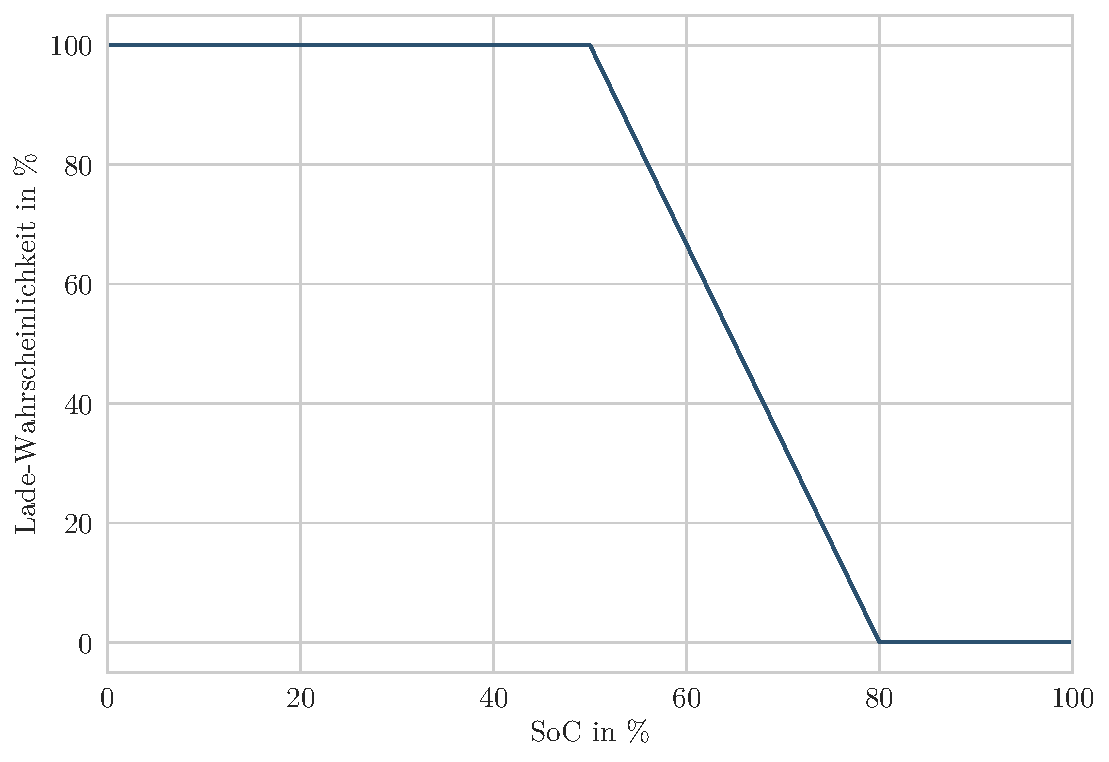
\includegraphics[width=0.9\textwidth]{Bilder/soc_charging_prob}
    \caption{Abhängigkeit der Ladewahrscheinlichkeit vom SoC an öffentlichen Standorten}\label{fig:soc_charging_prob}
\end{figure}

Schnellladeinfrastruktur besitzt aufgrund des zusätzlichen Fahrt- und Zeitaufwandes eine geringe Attraktivität für den Nutzer.
Deshalb wird eine Schnellladung in dieser Simulation nur dann ausgelöst, wenn es wirklich nötig ist.
Sinkt der \gls{SOC} eines Fahrzeugs unter \SI{20}{\percent}, wird eine Schnellladestation angefahren und das Fahrzeug für \SI{15}{\Minuten} geladen.
Im Unterschied zu \glspl{BEV} können \glspl{PHEV} auch mit einem \gls{SOC} von \SI{0}{\percent} ihre Fahrt mit Hilfe des Verbrennungsmotors fortsetzen.
Aus diesem Grund wird bei \glspl{PHEV} kein Schnellladevorgang ausgelöst.


\subsubsection{Regionalisierung des Fahrzeugbestandes}

Um die Anzahl an Fahrzeugen je Netzgebiet zu bestimmen, muss der Gesamtbestand an Fahrzeugen je Szenario (s. \autoref{tab:SzenarienRampUp} und \autoref{tab:CarSplit}) regionalisiert werden.
Die Regionalisierung der Fahrzeuge findet vorerst auf Ebene der Landkreise statt.
Als Grundlage hierfür dient der aktuelle Fahrzeugbestand nach Zulassungsbezirken \cite[][Stand: \DTMdate{2020-01-01}]{KBAPLZ2020}.
Es wird davon ausgegangen, dass es zu keiner Verschiebung des Anteils am Bestand zwischen den Zulassungsbezirken kommt.
Dies bedeutet, dass die Gesamtanzahl der Fahrzeuge je Fahrzeugklasse je Szenario entsprechend des heutigen Bestandes anteilig verteilt wird.
Die Aufteilung der Fahrzeuge in Klassen erfolgt anhand der Einteilung des Fahrzeugsbestands in Hubraum-Klassen, welche ebenfalls dem Fahrzeugbestand nach Zulassungsbezirken entnommen werden können.\medskip

Die geographische Einteilung der Landfläche in \glspl{REGIOSTAR} erfolgt auf Gemeindeebene, weshalb eine weitere Regionalisierung der Fahrzeuge innerhalb eines Landkreises auf die jeweiligen Gemeinden nötig ist.
Da auf Gemeindeebene keine Daten zum Fahrzeugbestand vorliegen, erfolgt die Regionalisierung anhand der Bevölkerungszahl der Gemeinden.
Die Grundlage hierfür bildet der Datensatz \glqq Gemeindegrenzen 2017 mit Einwohnerzahl\grqq{} \cite[][Stand: \DTMdate{2017-12-31}]{EDG2020}.
Die Verteilung der Anzahl der Fahrzeuge erfolgt streng proportional zur Bevölkerungszahl in der jeweiligen Gemeinde.
Jedes \gls{MS}-Netzgebiet streckt sich dabei in der Regel über mehrere Gemeinden, wobei einzelne Gemeinden auch nur anteilig innerhalb eines Netzgebietes liegen können.\medskip

Um abschließend die Fahrtprofile erzeugen zu können, muss jeder Gemeinde eine \gls{REGIOSTAR} Nummer zugeordnet werden.
Die entsprechende Zuordnung für das Jahr \num{2018} kann dem Datensatz \glqq Referenzdateien zur regionalstatistischen Raumtypologie\grqq{} \cite[][Stand: \DTMdate{2018-01-01}]{BMVIa2020} entnommen werden.


\subsection{Räumliche Verteilung der Ladevorgänge}\label{chap:theo_distribution}

Die räumliche Verteilung der Ladevorgänge innerhalb eines geographischen Gebietes kann starken Einfluss auf die Auswirkungen der Netzintegration von \glspl{EPKW} haben.
So können beispielsweise regionale Konzentrationen von Ladepunkten einzelne Leitungen stark beanspruchen und den Netzausbaubedarf erhöhen.\medskip

Innerhalb dieser Arbeit erfolgt die Verteilung der Ladevorgänge immer innerhalb des untersuchten geographischen Gebietes.
In Realität wird es vorkommen, dass Fahrzeuge außerhalb ihres während der Regionalisierung zugewiesenen geographischen Gebietes geladen werden.
Dies betrifft vor allem den Pendel- und Urlaubsverkehr.
Ein Laden in anderen geographischen Gebieten oder das Laden von Fahrzeugen aus anderen Gebieten im untersuchten Gebiet kann nicht abgebildet werden.
Es wird davon ausgegangen, dass sich die hierdurch entstehende Verschiebung des Ladebedarfs zwischen den einzelnen Gebieten ungefähr ausgleicht und keinen großen Einfluss auf die Ergebnisse dieser Untersuchung hat.
Es ist vorstellbar, dass in einzelnen Fällen auch größere Verschiebungen entstehen, wenn z.B. innerhalb eines geographischen Gebietes ein großer Ladepark aufgebaut wird, der als Anlaufpunkt für eine Vielzahl von Fahrzeugen aus anderen Gebieten dient. 
Ein solcher Fall kann somit nicht innerhalb dieser Arbeit abgebildet werden.\medskip

Grundlage für die Ermittlung von möglichen Standorten mitsamt einer Gewichtung der Standorte bietet eine geoinformatische Auswertung der untersuchten geographischen Gebiete.
Das hierfür verwendete Software Tool wird unabhängig von dieser Arbeit am Reiner Lemoine Institut entwickelt und ist noch nicht veröffentlicht.
Erweiternd zu der Identifizierung der möglichen Ladeinfrastruktur wurde innerhalb dieser Arbeit eine Methodik für die Zuteilung der Ladevorgänge auf die Ladeinfrastruktur entwickelt.


\paragraph{Private Ladeinfrastruktur:}

Die private Ladeinfrastruktur beinhaltet alle Ladevorgänge, die an privater Ladeinfrastruktur am Eigenheim, in Wohnanlagen oder auf dem Firmenparkplatz stattfinden.
Um mögliche Standorte für die Ladeinfrastruktur am Eigenheim oder in Wohnanlagen identifizieren zu können, wird die Anzahl an Wohneinheiten auf einem \SI{100 x 100}{\m} Raster aus dem Zensus 2011 \cite{StatistischesBundesamt2011} verwendet.
So wird jedem Raster mit mehr als einer Wohneinheit und einer Einwohnerzahl größer Null ein möglicher Anschlusspunkt für Ladeinfrastruktur zugeordnet und anhand der Gesamtanzahl von Wohneinheiten im Raster gewichtet. \medskip

Für private Ladeinfrastruktur auf Firmenparkplätzen werden die Klassifizierungen der Landflächen nach Nutzungsart nach der \gls{OSM} \cite{OpenStreetMapFoundation} verwendet.
Hierbei wird jeder Landfläche mit der Nutzungsart \glqq commercial\grqq , \glqq retail\grqq{} oder \glqq industrial\grqq{} ein möglicher Anschlusspunkt für Ladeinfrastruktur zugeordnet.
Die Gewichtung erfolgt anhand der Fläche des Gebietes multipliziert mit einem Flächennutzungsfaktor.
Der Flächennutzungsfaktor liegt für \glqq commercial\grqq{} bei \num{3}, für \glqq retail\grqq{} bei \num{2} und für \glqq industrial\grqq{} bei \num{1}.


\paragraph{Öffentliche Ladeinfrastruktur:}

Die öffentliche Ladeinfrastruktur beinhaltet Ladeinfrastruktur, die nicht der privaten Ladeinfrastruktur zugeordnet werden kann.
Grundsätzlich lässt sich hierbei zwischen Normal- und Schnellladeinfrastruktur unterscheiden.
Für die Normalladeinfrastruktur wird allen \glspl{POI} aus der \gls{OSM} \cite{OpenStreetMapFoundation} in dem untersuchten Gebiet jeweils ein möglicher Anschlusspunkt für Ladeinfrastruktur zugeordnet.
Die Gewichtung der Anschlusspunkte erfolgt hierbei anhand der Gesamtanzahl an \glspl{POI} in der Nähe des Anschlusspunktes.\medskip

Für Schnellladeinfrastruktur wird jeder Tankstelle aus der \gls{OSM} \cite{OpenStreetMapFoundation} im untersuchten Gebiet jeweils ein Anschlusspunkt zugeordnet.
Liegt innerhalb des Gebietes keine Tankstelle, so wird ein zufälliger Anschlusspunkt der öffentlichen Ladeinfrastruktur verwendet.
Eine Gewichtung findet in diesem Fall nicht statt.


\paragraph{Zuteilung der Ladevorgänge auf die Ladeinfrastruktur:}

Bei der Ladeinfrastruktur auf Firmenparkplätzen werden sehr große Flächen identifiziert, die in der Regel nicht nur einem Arbeitgeber zugewiesen werden können.
Da hierdurch unter Umständen nur wenige Anschlusspunkte generiert werden, werden ergänzend \SI{50}{\percent} der möglichen öffentlichen Normalladeinfrastruktur zusätzlich für Ladeinfrastruktur am Arbeitsplatz genutzt.
Den zusätzlichen Anschlusspunkten wird eine geringe Gewichtung zugeordnet, da durch diese vor allem kleine Betriebe abgebildet werden sollen.
Die Gewichtung orientiert sich dabei an der ermittelten Gewichtung der öffentlichen Ladeinfrastruktur.
Bei der privaten Ladeinfrastruktur am Eigenheim oder in Wohnanlagen liegen innerhalb eines Rasters in der Regel mehrere Wohneinheiten, weshalb davon auszugehen ist, dass je identifiziertem Anschlusspunkt mehrere unabhängige Ladepunkte bzw. -parks betrieben werden.
Und auch bei der öffentlichen Normalladeinfrastruktur können unter Umständen durchaus mehrere unabhängige Ladepunkte bzw. -parks betrieben werden.
Deshalb werden in diesen drei Fällen die möglichen Anschlusspunkte mehrfach vergeben.
Dabei wird für die Ladeinfrastruktur am Eigenheim oder in Wohnanlagen ein Belegungsfaktor von \num{7}, für die Ladeinfrastruktur auf Firmenparkplätzen von \num{5} und für die öffentlichen Normalladeinfrastruktur von \num{2} verwendet.\medskip

Jedem Anschlusspunkt wird vor der Zuteilung der Ladevorgänge eine maximale Anzahl an möglichen Ladepunkten zugeordnet.
Diese entspricht dem Verhältnis von Fahrzeugen im Netzgebiet und der Anzahl von möglichen Ladepunkten je \UC multipliziert mit einem Faktor von \num{5}.
Nachdem einem Anschlusspunkt ein Ladepunkt zugeordnet wird, wird die Gewichtung des Anschlusspunktes linear abgesenkt, sodass die Gewichtung des Anschlusspunktes auf Null fällt, sobald die maximale Anzahl an möglichen Ladepunkten erreicht wurde.\medskip

Die Zuteilung der Ladevorgänge auf die Ladeinfrastruktur erfolgt mit Hilfe des Gewichtungsfaktors der Anschlusspunkte.
Dabei erfolgt eine zufällige und gewichtete Auswahl eines Anschlusspunktes je Ladevorgang.
Im Falle der privaten Ladeinfrastruktur wird für jedes Fahrzeug ein eigener Ladepunkt eingerichtet.
Diesem Ladepunkt werden alle Ladevorgänge des jeweiligen Fahrzeuges und \UCs zugeordnet.\medskip

Für die öffentliche Ladeinfrastruktur erfolgt die Zuweisung dezidiert pro Ladevorgang.
So wird je Ladevorgang untersucht, ob bereits ein passender Ladepunkt zur Verfügung steht.
Hierbei wird beachtet, ob in dem entsprechenden Zeitraum der Ladepunkt durch ein anderes Fahrzeug besetzt ist und ob der Ladepunkt die entsprechende Ladeleistung zur Verfügung stellen kann.
Sollte kein passender Ladepunkt zur Verfügung stehen, wird analog zum Vorgehen bei der privaten Ladeinfrastruktur ein Ladepunkt zufällig und gewichtet ausgewählt und eingerichtet.\medskip

Da die \gls{MS}-Netzgebiete nicht immer die Gesamtfläche einer Gemeinde abdecken, muss abschließend geprüft werden, ob die generierten Anschlusspunkte innerhalb des Netzgebietes liegen.
Liegt ein Anschlusspunkt innerhalb eines \gls{MS}-Netzgebietes, so wird er diesem zugeordnet.
Tut dieser es nicht, dann entfallen die zugeordneten Ladevorgänge auf ein angrenzendes Netzgebiet und sind somit nicht Teil der abschließenden Auswertungen.


\paragraph{Netzintegration der Ladeinfrastruktur:}

Die Netzintegration der Ladeinfrastruktur erfolgt automatisiert mit Hilfe der \textit{integrate\_component} Funktionalität \glspl{EDISGO}.
Der Anschluss erfolgt hierbei bis zu einer Anschlussleistung von \SI{0.3}{\mva} in der Niederspannung und darüber direkt in der Mittelspannung.

{\color{red} TODO: @Birgit: Sollte ich hier noch mehr schreiben? Wenn ja was?}


\subsection{Ladestrategien}\label{chap:theo_strategies}

Innerhalb dieser Arbeit werden zwei präventive Ladestrategien und eine aktive Ladestrategie untersucht.
Auf diese Weise soll untersucht werden, inwieweit eine aktive Ladestrategie gegenüber präventiven Ladestrategien Vorteile aufweist.
Da für aktive Ladestrategien der Aufwand im Betrieb höher ist und zusätzliche Technik benötigt wird, liegen die Kosten für solche Ladestrategien deutlich höher.\medskip

Das Ziel der Ladestrategien ist es, ein möglichst netzfreundliches Verhalten der Ladevorgänge zu erzeugen, ohne den Komfort für Endverbraucher$^*$innen einzuschränken.
Deshalb gilt als Randbedingung aller Ladestrategien, dass der Ladebedarf jedes Ladevorgangs zu \SI{100}{\percent} gedeckt werden muss.
Dies bedeutet, dass Ladevorgänge nur dann flexibilisiert werden können, wenn innerhalb der Standzeit eine Vollladung des Fahrzeuges möglich ist.
Weiterhin können nur private Ladevorgänge flexibilisiert werden, da bei öffentlichen Ladevorgängen die Erfüllung der Dienstleistung im Vordergrund steht.
Um die drei Ladestrategien bewerten zu können, wird zusätzlich eine Referenz-Ladestrategie untersucht.


\paragraph{Referenz-Laden:}

Bei der Referenz-Ladestrategie wird für Ladevorgänge in der \gls{NS}-Ebene ein vollkommen ungesteuertes Laden der Fahrzeuge angenommen.
Da bei großen privaten Ladeparks ein ungesteuertes Laden als unrealistisch einzuschätzen ist, wird davon ausgegangen, dass ab einem Anschluss in der \gls{MS}-Ebene der Betreiber eine Reduktion der Spitzenlast anstrebt.
In diesen Fällen kommt auch bei der Referenz-Ladestrategie das reduzierte Laden zum Einsatz, welches anschließend erläutert wird.


\paragraph{Ladegruppen:}

Das Ziel der Ladegruppen ist es, die Netzbelastung präventiv durch die Senkung der Gleichzeitigkeit der Ladevorgänge zu reduzieren.
Hierfür werden die einzelnen Ladepunkte in zwei Gruppen eingeteilt.
Beiden Gruppen werden alternierend 15-minütige Ladezeitfenster zugewiesen, in denen bei voller Ladeleistung der Ladebedarf gedeckt wird.
Reichen die zugewiesenen Ladezeitfenster nicht aus, um den Ladebedarf des Ladevorgangs zu decken, werden auch die Ladezeitfenster der anderen Gruppe verwendet bis der Ladebedarf gedeckt werden kann.
Die Ladezeitfenster der eigenen Gruppe werden dabei priorisiert behandelt.
Es wird darauf geachtet, dass die Zuweisung der Gruppen nicht nur innerhalb eines Netzgebietes ausgeglichen erfolgt, sondern detailliert bis in die einzelnen Stränge der \gls{NS}-Ebene.
Innerhalb eines \gls{NS}-Stranges wird weiterhin darauf geachtet, dass auch die einzelnen Leistungsklassen der Ladeinfrastruktur gleichmäßig auf die Gruppen verteilt werden.
In \autoref{fig:group_vis} findet sich eine beispielhafte Einteilung von Ladepunkten auf die zwei Gruppen innerhalb eines \gls{NS}-Stranges.

\begin{figure}[H]
    \centering
    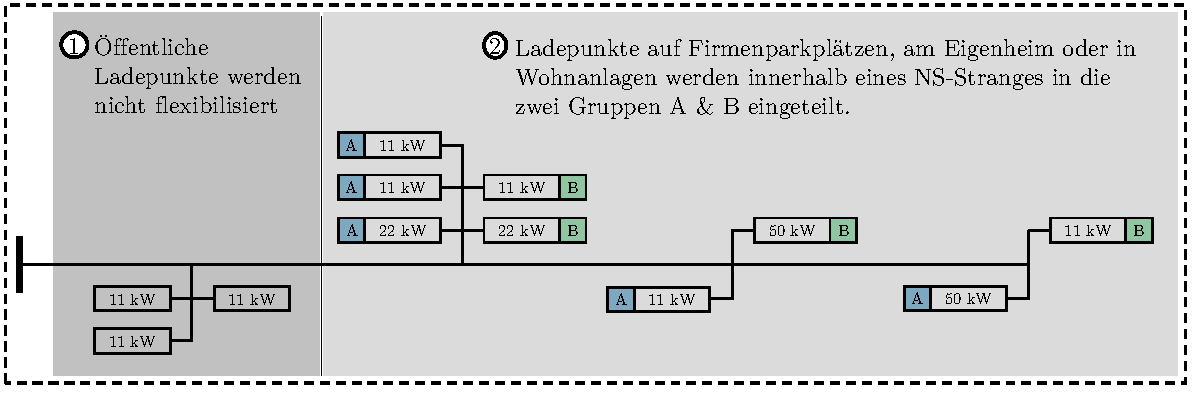
\includegraphics[width=\textwidth]{Bilder/grouped_charging_vis_cropped}
    \caption{Einteilung der Ladepunkte eines NS-Stranges in die Gruppen A \& B für das gruppierte Laden}\label{fig:group_vis}
\end{figure}


\paragraph{Reduziertes Laden:}

Im Gegensatz zu den Ladegruppen soll beim reduzierten Laden die Senkung der Netzbelastung präventiv durch die Reduzierung der Ladeleistung der einzelnen Ladevorgänge erreicht werden.
Hierbei wird durch eine Absenkung der Ladeleistung möglichst die gesamte Standzeit des Fahrzeuges für den Ladevorgang ausgenutzt.
Die Flexibilität dieser Ladestrategie wird durch eine Mindestladeleistung von \SI{10}{\percent} der Nennleistung des angefahrenen Ladepunktes technisch begrenzt.
Hierdurch soll ein Kompromiss zwischen einer möglichst großen Reduktion der Ladeleistung und den technischen Anforderungen der Ladeinfrastruktur gefunden werden.
Im Gegensatz zur Referenz-Ladestrategie werden unabhängig von der Netzebene beim reduzierten Laden alle privaten Ladevorgänge flexibilisiert.

% TODO: Quelle Konferenzpaper Birgit?


\paragraph{Residuallast-Laden:}

Bei dem Residuallast-Laden handelt es sich um eine aktive Ladestrategie.
Der Ladevorgang eines Fahrzeuges findet hierbei immer innerhalb der Zeitpunkte der Standzeit statt, welche die geringste Residuallast innerhalb des Netzgebietes aufweisen, wodurch eine Glättung der Residuallast erreicht werden soll.
Die Zuweisung findet auf Viertelstundenbasis statt und die Ladevorgänge finden immer bei voller Ladeleistung statt.
Das Ziel der Optimierung kann so formuliert werden, dass eine Minimierung der \glspl{MQA} nach \autoref{eq:residual} der Residuallast vom Mittelwert der Residuallast angestrebt wird.

\begin{equation}
	\text{MQA} = \frac{1}{n} \sum_i^n \left( P_{\text{R}_i} - \overline{P}_{\text{R}} \right)^2
	\label{eq:residual}
\end{equation}

\noindent Wobei:

\addvbuffer[12pt 12pt]{
	\begin{tabular}{>{$}r<{$}@{\ :\ }l}
		P_{\text{R}_i}				& Residuallast zum Zeitschritt $i$  \\
		\overline{P}_{\text{R}}		& Mittelwert der Residuallast 		\\
		n							& Anzahl an Zeitschritten			\\
		i							& Index des Zeitschrittes 			\\
	\end{tabular}
}

Durch die Abhängigkeit der Residuallast von den einzelnen Ladevorgängen sind auch die Ergebnisse der Optimierung der einzelnen Ladevorgänge voneinander abhängig.
Hierdurch entsteht ein komplexes Optimierungsproblem.
Um die Rechenzeit in einem akzeptablen Maß zu halten, wird eine Näherung an eine optimale Lösung angestrebt.
So wird für jeden Ladevorgang ermittelt, wie viel überschüssige Standzeit zur Flexibilisierung der Ladevorgänge zur Verfügung steht.
Die Ladevorgänge werden anschließend in Abhängigkeit dieses Kriteriums in aufsteigender Reihenfolge sortiert und einzeln betrachtet.
So werden für jeden Ladevorgang die nötigen Zeitschritte für den Ladevorgang ausgewählt, die innerhalb der Standzeit die geringste Residuallast aufweisen.
Zusätzlich wird die Residuallast entsprechend angepasst und somit die Abhängigkeit der einzelnen Ladevorgänge voneinander gewährleistet.
Auf diese Weise werden Ladevorgänge mit einem geringen Flexibilitätsband vorrangig behandelt und eine möglichst optimale Lösung bei einem geringen Rechenaufwand erreicht.


\subsection{Netzuntersuchung}\label{chap:edisgo_theo}

Das Open Source Tool \gls{EDISGO} stellt eine Toolbox zur Verfügung, um Verteilnetze auf Netzprobleme zu untersuchen.
Gleichzeitig können mit \gls{EDISGO} Maßnahmen zur Behebung der Netzprobleme bewertet werden.
Dabei bilden synthetische Netztopologien, die mit Hilfe des Open Source Tools \gls{DINGO} erzeugt wurden, die Grundlage für die Berechnungen mit \gls{EDISGO}.
\gls{EDISGO} kann über GitHub \cite{edisgoGit2019} abgerufen werden und ist auf Read the Docs \cite{edisgoDocs2017} dokumentiert.
Innerhalb dieses Kapitels werden die wichtigsten Funktionalitäten \glspl{EDISGO} für die Durchführung der Berechnungen innerhalb dieser Masterarbeit dargestellt und erläutert.


\paragraph{Ermittlung von Netzproblemen:}\label{chap:grid_issues}

Die Überprüfung der einzelnen Netze auf Netzprobleme erfolgt in zwei Schritten.
Vorerst wird eine nichtlineare Lastflussberechnung durchgeführt, um anschließend die Einhaltung der Spannungsanforderungen und technischen Richtlinien bezüglich der Betriebsmittelbelastungen zu überprüfen.
Die Durchführung der Lastflussberechnung erfolgt mit Hilfe des Open Source Tools \textit{PyPSA} \cite{Brown2020}.
In diesem Kapitel soll auf die theoretischen Grundlagen der Lastflussberechnung, den Umfang der Analyse und die Spannungsanforderungen und technischen Richtlinien bezüglich der Gerätebelastungen eingegangen werden.\medskip

Das Ziel der Lastflussberechnung ist es, das zwischen allen Verbindungen der Netzknoten $i$ und $k$ die folgende Gleichung erfüllt wird:

\begin{equation}
	S_i = P_i + j Q_i = V_i I_i^* = V_i \left(\sum_j Y_{i,k} V_k \right)^*
	\label{eq:pf}
\end{equation}

\noindent Wobei:

\addvbuffer[12pt 12pt]{
	\begin{tabular}{>{$}r<{$}@{\ :\ }l}
		S_i 		& Scheinleistung am Netzknoten $i$ \\
		P_i	 		& Wirkleistung am Netzknoten $i$ \\
		Q_i			& Blindleistung am Netzknoten $i$ \\
		V_i			& Komplexe Spannung am Netzknoten, wobei $V_i = \left| V_i \right|e^{j \theta_i}$ \\
		I_i			& Stromstärke am Netzknoten \\
		Y_{i,k}		& Admittanz der Leitung zwischen den Netzknoten $i$ und $k$ \\
	\end{tabular}
}

% TODO: von Birgit mal erklären lassen^^

Der Winkel der komplexen Spannung ist relativ zum Bilanzknoten.
Unter dem Bilanzknoten wird ein Netzknoten verstanden, an welchem der Wirk- und Blindleistungsfluss frei eingestellt werden kann.
Mit Hilfe des Bilanzknotens kann über einen iterativen Prozess die Konvergenz nach \autoref{eq:pf} des Systems erreicht werden.
Eine genau Beschreibung der Lastflussberechnung des Open Source Tools \textit{PyPSA} kann auf Read the Docs \cite{Brown2020a} abgerufen werden.
Da die Spannung der Sekundärseite des \gls{HS}-\gls{MS}-\glspl{USW} eingestellt werden kann, eignet sich dieser Punkt besonders gut und wird innerhalb dieser Masterarbeit als Bilanzknoten verwendet.
Alle weiteren Netzknoten werden mit gegebenen Wirk- und Blindleistungen modelliert. \cite{Schachler}\medskip

Die Lastflussanalyse der Netze berücksichtigt sowohl \gls{MS}- und \gls{NS}-Leitungen als auch die \gls{MS}-\gls{NS}-Umspannebene.
Gegenüber einer Aggregation der Erzeugung und des Bedarfes der einzelnen \gls{NS}-Netze an dem jeweiligen \gls{MS}-\gls{NS}-\gls{USW} bietet diese besonders tiefgehende Betrachtung die Möglichkeit, die Auswirkungen der teilweise hohen Ladeleistungen der Ladeinfrastruktur genauer zu betrachten und den Einfluss verschiedener Ladestrategien umfassender bestimmen zu können.
Da die Sekundärseite des \gls{HS}-\gls{MS}-\glspl{USW} als Bilanzknoten modelliert wird, können an dieser keine Spannungsprobleme auftreten.
Jedoch entspricht die Scheinleistung des Bilanzknotens der Leistung, die über das \gls{HS}-\gls{MS}-\gls{USW} geleitet wird.
Anhand dieses Wertes können zusätzlich Aussagen über die Belastung des \gls{HS}-\gls{MS}-\glspl{USW} getroffen werden. \cite{Schachler}\medskip

Mit Hilfe der durch die Lastflussanalyse ermittelten Belastungen und Spannungsabweichungen an den Betriebsmitteln können abschließend Überlastungen und Spannungsprobleme festgestellt werden.
Die zulässigen Belastungsfaktoren und Spannungsabweichungen finden sich in \autoref{chap:theo_grid}.
In \autoref{fig:scope} findet sich eine Übersicht über den Umfang der Lastflussanalyse.

\begin{figure}[H]
    \centering
    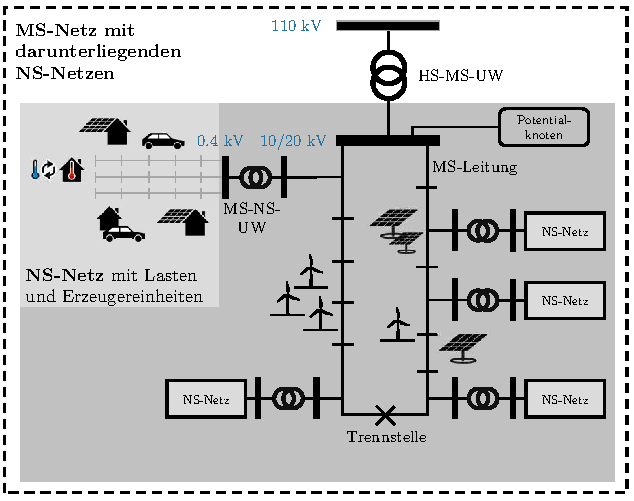
\includegraphics[width=\textwidth]{Bilder/scope_power_flow_kh_cropped}
    \caption[Umfang der Lastflussanalyse mit eDisGo]{Umfang der Lastflussanalyse mit eDisGo \cite{Schachler}}\label{fig:scope}
\end{figure}


\paragraph{Ermittlung des Abregelungsbedarfs für die Auflösung von Netzüberlastungen:}

Die Ermittlung des Abregelungsbedarfs für die Auflösung von Spannungsbandverletzungen und Betriebsmittelüberbelastungen erfolgt in einem iterativen Prozess.
Vorerst werden etwaige Netzprobleme und die entsprechenden Zeitschritte, in denen die Netzprobleme auftreten, mit Hilfe der zuvor beschriebenen Lastflussanalyse ermittelt.
Anschließend wird die Last bzw. die Einspeisung in Schritten von \SI{10}{\percent} innerhalb der ermittelten Zeitschritte reduziert.
Die beiden Schritte werden so lange wiederholt bis keine Netzprobleme mehr auftreten.\medskip

Um die Rechenzeit innerhalb eines akzeptablen Maßes zu halten, erfolgt die Ermittlung des Abregelungsbedarfs für zwei Wochen des Jahres.
Hierbei werden die Wochen untersucht, die im Netzgebiet die minimale bzw. maximale durchschnittliche Residuallast aufweisen.
Auf diese Weise sollen möglichst extreme Belastungssituationen abgedeckt werden.\medskip

Aufgrund der hohen Anzahl an \glspl{EPKW}, \glspl{WP} und erneuerbaren Erzeugereinheiten kommt es in einigen Fällen dazu, dass die Lastflussanalyse nicht konvergiert.
Dabei werden zuerst die einzelnen \gls{NS}-Netzgebiete eines \gls{MS}-Netzgebietes einzeln betrachtet, um dort extreme Belastungssituationen abzufangen, die eine Konvergenz des Gesamtsystems verhindern können.
Durch die vorgeschaltete Einzelbetrachtung der \gls{NS}-Netzgebiete kann der Abregelungsbedarf eindeutig der \gls{NS}- bzw. \gls{MS}-Ebene zugeordnet werden.\medskip

Bei der Lösung der Netzprobleme werden vorerst Spannungsprobleme und abschließend Überlastungen gelöst.
Weiterhin werden Probleme in der \gls{NS}-Ebene gelöst, bevor Probleme in der \gls{MS}-\gls{NS}-Umspannebene und abschließend in der \gls{MS}-Ebene gelöst werden.
Durch die Lösung von Netzproblemen auf tieferen Spannungsebenen können unter Umständen bereits Netzprobleme in darüber liegenden Spannungsebenen gelöst oder entspannt werden.
Weiterhin werden Netzprobleme innerhalb der \gls{NS}- bzw. \gls{MS}-Ebene anhand ihrer Entfernung zur übergeordneten Umspannebene priorisiert.
So kann auch hier die Lösung von weiter entfernten Netzproblemen bereits vorgeschaltete Netzprobleme auflösen oder entspannen.
Für jeden Zeitschritt, in dem Überlastungs- oder Spannungsprobleme an einem Netzknoten auftreten, wird geprüft, ob die Netzprobleme durch hohe Nachfrage oder hohe Einspeisung entstehen.
Anhand dieser Information wird entscheiden, ob Last oder Einspeisung abgeregelt werden soll.\medskip

Die gesamte notwendige Abregelung für das \gls{MS}-Netz ergibt sich aus der Summierung aller nötigen Abregelungen von Last und Erzeugung.
In \autoref{fig:scope_curtailment} findet sich eine Veranschaulichung des Vorgehens.

\begin{figure}[H]
    \centering
    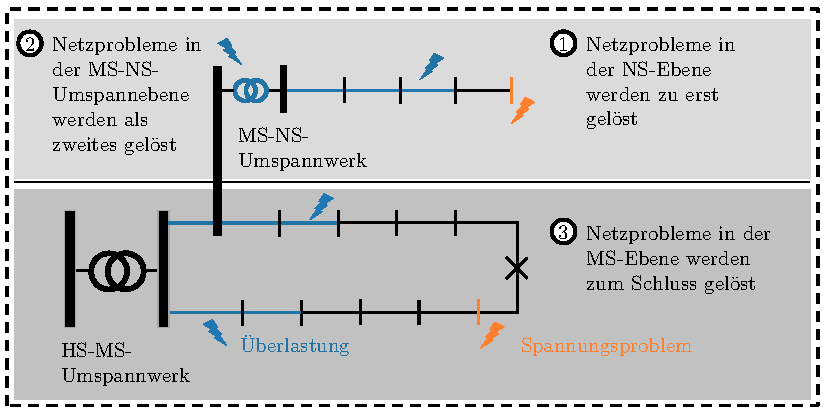
\includegraphics[width=\textwidth]{Bilder/grid_issues_scope_cropped}
    \caption[Umfang der Ermittlung des Abregelungsbedarfs für die Auflösung von Spannungsbandverletzungen und Betriebsmittelüberbelastungen]{Umfang der Ermittlung des Abregelungsbedarfs für die Auflösung von Netzüberlastungen \cite{Schachler}}\label{fig:scope_curtailment}
\end{figure}

